\chapter{Конструкторский раздел}
\section{Декомпозиция задачи на верхнем уровне}
На верхнем уровне (рис.~\ref{fig:common}) задача может быть сформулирована как задача ранжирования источников по степени доверия к новостям, публикуемых данными источниками. На вход разрабатываемого алгоритма поступает список новостных лент и экспертная оценка достоверности некоторых новостей. На выходе же ожидается рейтинги источников для данного временного среза новостей.

\begin{figure}[h]
    \centering
    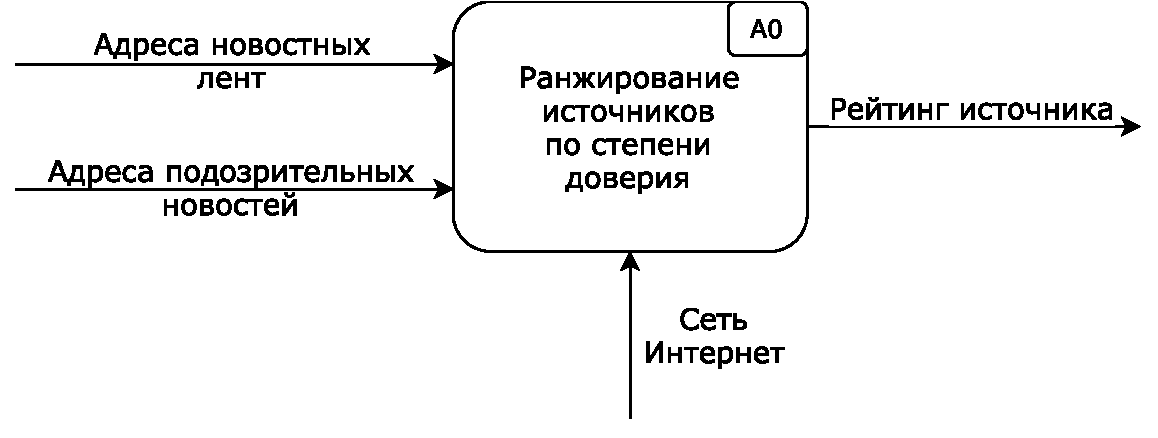
\includegraphics[width=.8\textwidth]{common.pdf}
    \caption{Постановка задачи.}
    \label{fig:common}
\end{figure}

\begin{figure}[h]
    \centering
    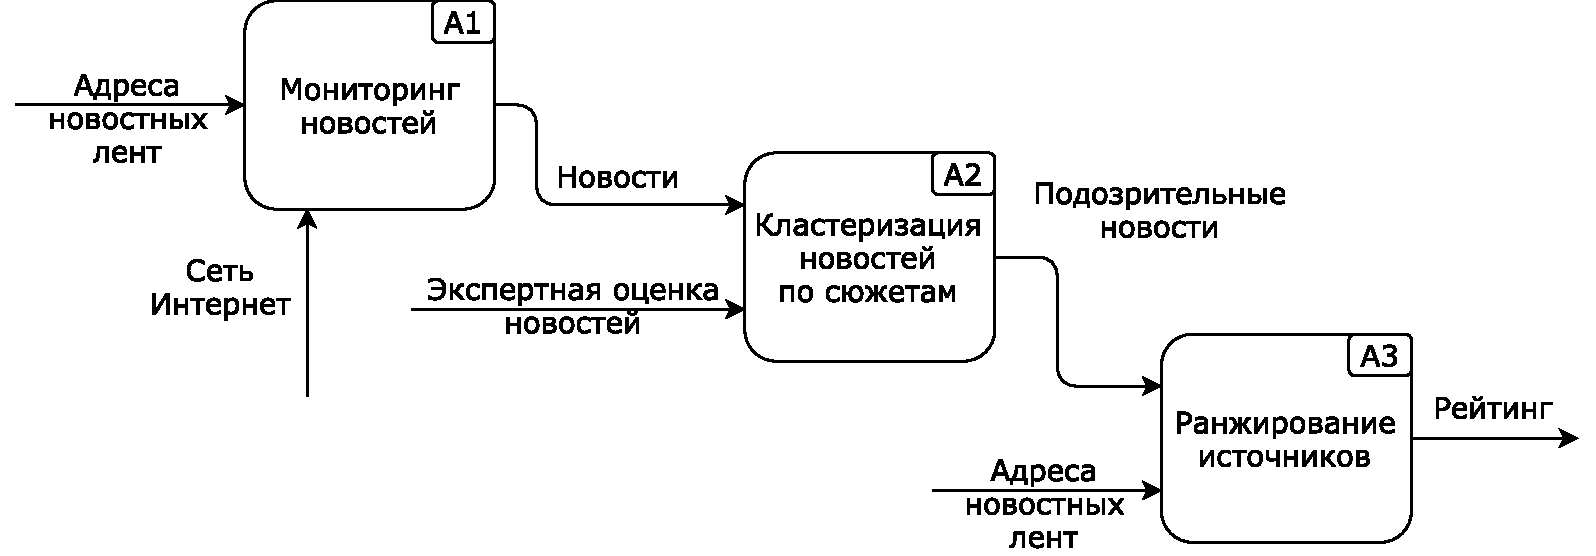
\includegraphics[width=\textwidth]{stages.pdf}
    \caption{Этапы решения задачи.}
    \label{fig:stages}
\end{figure}

В результате декомпозиции выделяются три основных этапа решения задачи (рис.~\ref{fig:stages}):
\begin{enumerate}
    \item Мониторинг потока новостей в реальном времени. Разрабатываемая система должна регулярно проверять наличие новых новостей по заданному набору rss/atom-лент, используя сетевой стек для доступа в глобальную сеть <<Интернет>>;
    \item Кластеризация новостей с последующим распространением оценки экспертов (то есть информации о том, какие новости и с какой вероятностью признаются недостоверными) достоверности новостей на другие новости внутри сюжета;
    \item Ранжирование источников, используя полученный список недостоверных новостей по каждому источнику.
\end{enumerate}

Перейдём к рассмотрению потоков данных в системе для выделенных этапов (рис.~\ref{fig:dataflows}).
\begin{figure}[h]
    \centering
    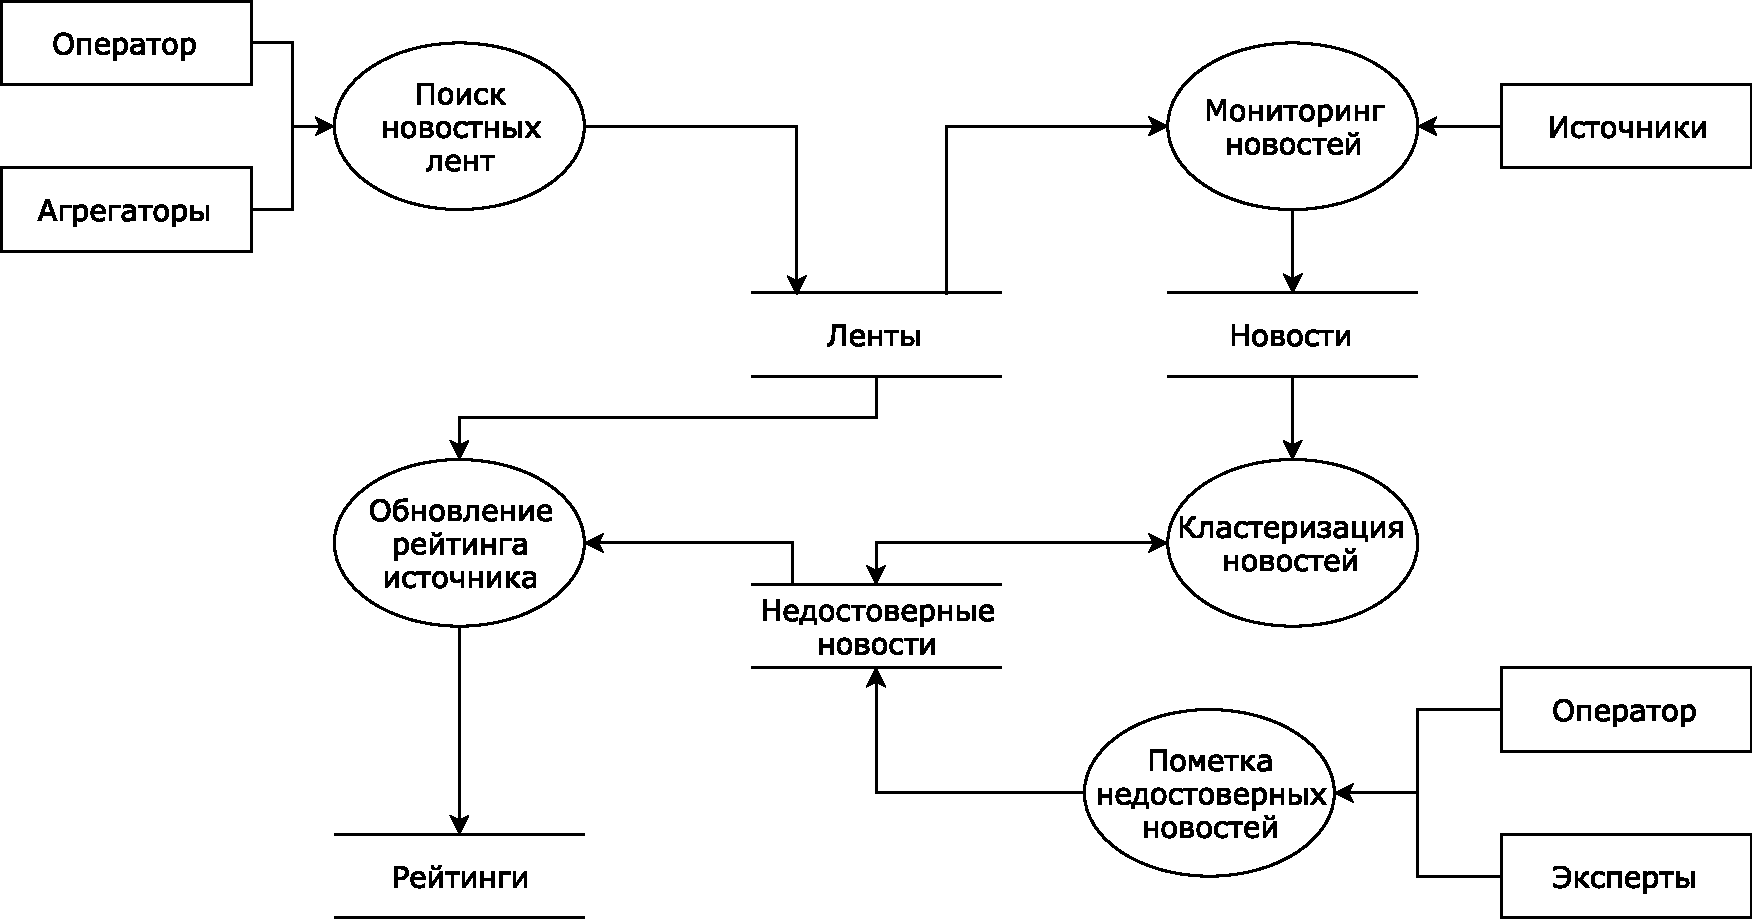
\includegraphics[width=\textwidth]{dataflows.pdf}
    \caption{Потоки данных в системе.}
    \label{fig:dataflows}
\end{figure}

Типы данных в системе:
\begin{itemize}
    \item Ленты~--- адреса rss/atom-лент и текущий период их обновления. В систему ленты попадают ручным добавлением со стороны оператора. Кроме того, периодически опрашиваются rss-агрегаторы (например feedly.com) на предмет появление новых популярных источников в заданных категориях (политика, экономика и другие);
    \item Новости~--- тексты новостей. В систему добавляются посредством регулярного опроса новостных лент и выкачивания новых статей со сайта источника;
    \item Недостоверные новости~--- адреса недостоверных новостей и оценки степени их недостоверности. В систему заносятся оператором и регулярно выкачиваются с экспертного сайта stopfake.org, а также в результате пометки схожих новостей;
    \item Рейтинги~--- рейтинги источников, обновляются при каждом появлении оценки очередной недостоверной новости.
\end{itemize}

\section{Мониторинг новостей}
Рассмотрим подробнее первый этап метода~--- мониторинг новостей (рис.~\ref{fig:raider}) в реальном времени.

\begin{figure}[h]
    \centering
    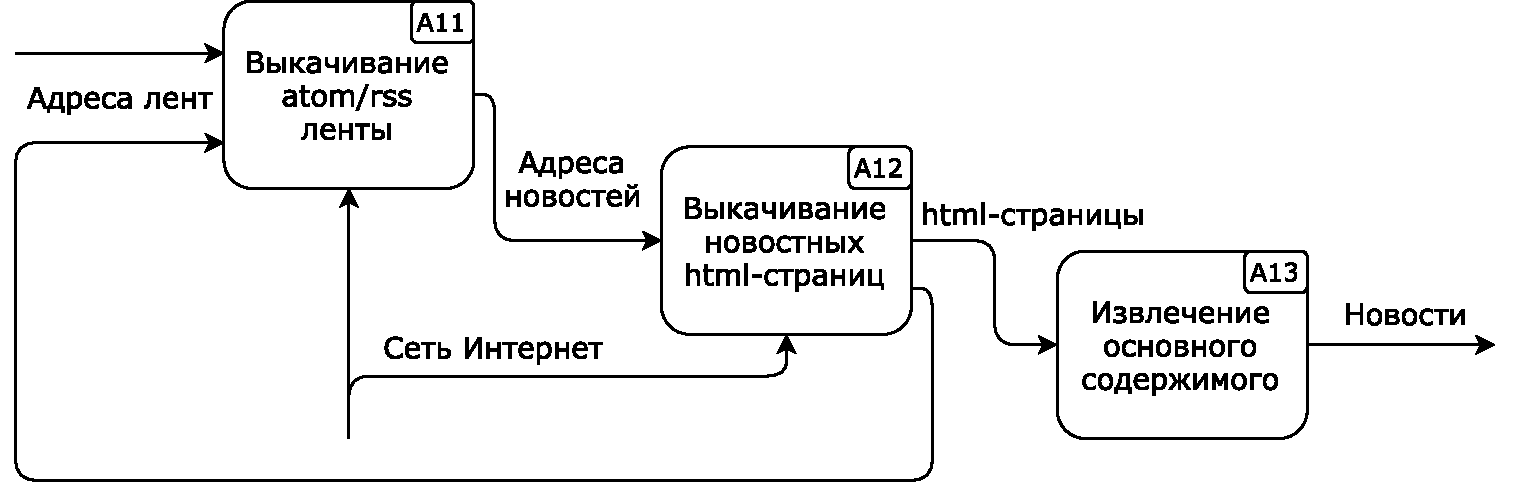
\includegraphics[width=\textwidth]{raider.pdf}
    \caption{Мониторинг новостей.}
    \label{fig:raider}
\end{figure}

Задачей данного этапа является регулярное получение новых новостей по списку rss/atom-лент. Для решения данной задачи используются методы и оптимизации из раздела~\ref{sec:collecting}.

\subsection{Выкачивание новостных лент}
Вместе с новостной лентой в системе хранится информация о дате последней новости, полученной по данной ленте, а так же вычисленный текущий период обновления ленты.

Так как одна и та же новость может быть доступна из нескольких лент, то необходимо фильтровать посещённые новости. Для этого используется фильтр Блума, описанные в разделе \ref{sssec:bloom-filter}.

Отдельной проблемой является определение периода обновления ленты, который зависит не только от частоты публикации новостей источником, но и политической ситуации и даже от времени суток.

Решить данную проблему можно следующим образом: при каждом получении ленты будем определять долю старых новостей в ней: $s$. Далее, определим некоторую константу $p$, определяющую идеальное значение такой доли. Если при очередном выкачивании ленты старых новостей стало больше, то необходимо увеличить период хождения за лентой, если же доля упала, то, наоборот, увеличить:
\begin{equation}
    t_n=t_{n-1}\cdot(1-trust)+\left(\frac{s}{p}\right)\cdot trust,
\end{equation}
\begin{conditions}
    $t_n$ & период выкачивания ленты; \\
    $trust$ & доверие к коэффициенту (пропорционально числу новостей). \\
\end{conditions}

\subsection{Выкачивание новостных страниц}
После выкачивания ленты и определения адресов новых новостей необходимо выкачать эти самые новости. Проблема заключается в том, что новость получается не напрямую, а только в составе html-страницы, содержащей мусор в виде рекламы, навигации и так далее.

При запросе к серверам источника учитываются ограничения, указываемые сайтом источника в стандарте исключений для роботов (см.~\ref{ssec:robotstxt}).

\subsection{Извлечение новости из страницы}
На данном шаге из html-страницы получается непосредственно новость, используя алгоритм выделения основного содержимого со страницы, изложенный в \ref{sssec:readability}, а так же декодирование мнемоник HTML (см.~\ref{sssec:html-mnemonics}). В результате получаем новости, которые можно использовать на следующем этапе~--- кластеризации.

Новости идентифицируются по ключу, получаемого в результате нормализации URL (см.~\ref{sssec:url-normalization}).

\section{Кластеризация}
Задачей данного этапа является объединение новостей в сюжеты и распространение экспертной оценки внутри кластера (рис.~\ref{fig:compounder}).

\begin{figure}[h]
    \centering
    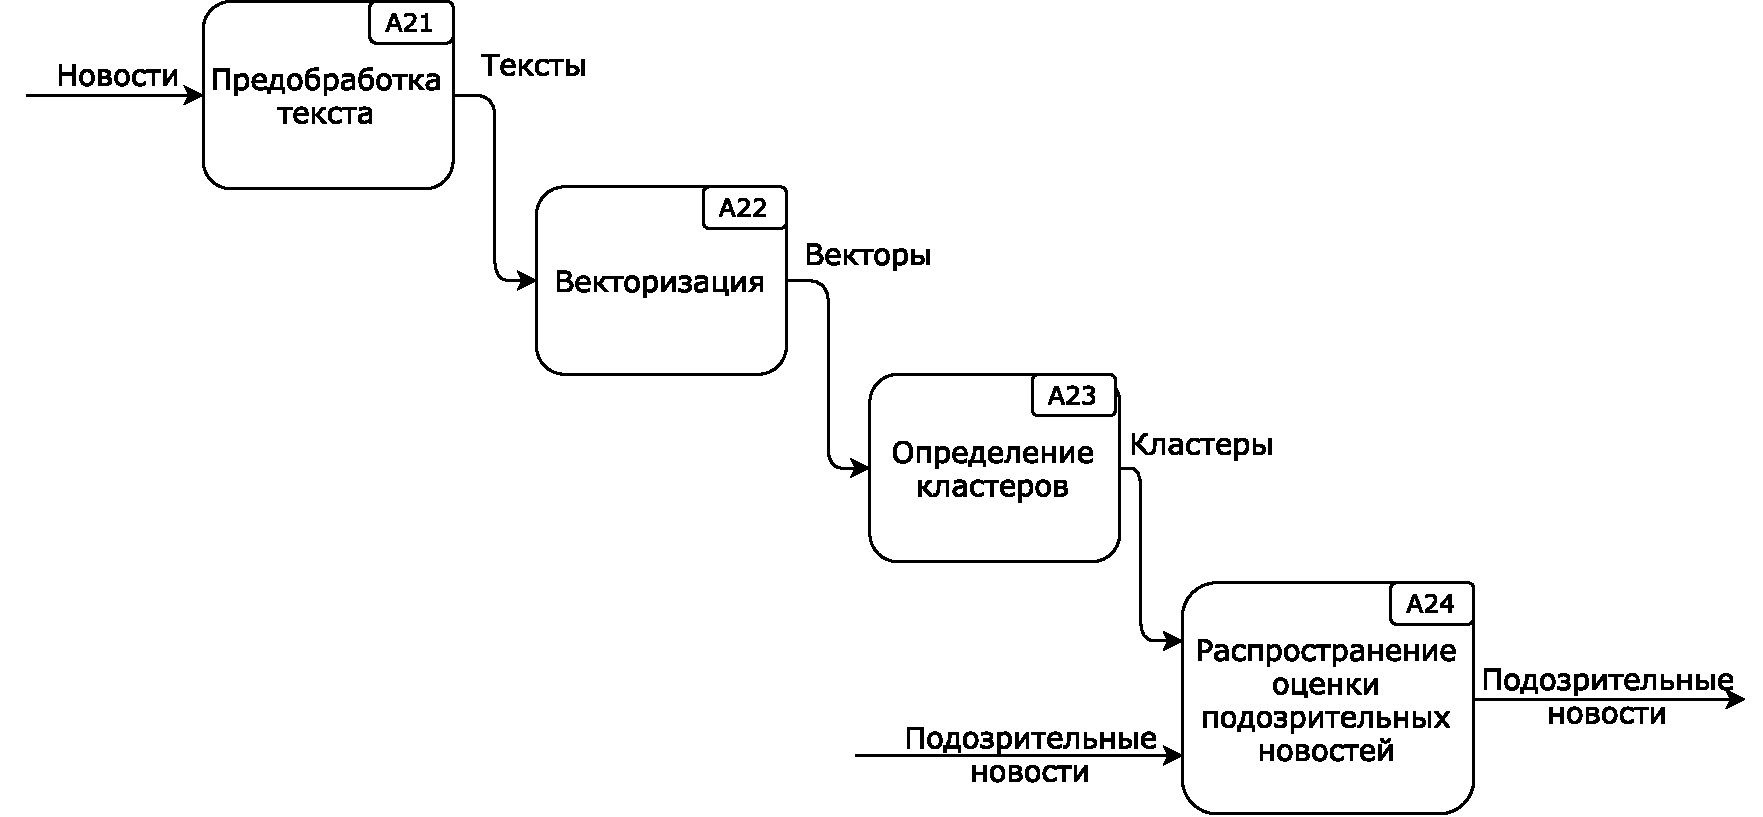
\includegraphics[width=\textwidth]{compounder.pdf}
    \caption{Кластеризация.}
    \label{fig:compounder}
\end{figure}

Рассмотрим подробнее шаги данного этапа.

\subsection{Предобработка}
Шаг предобработки текста включает в себя удаление стоп-слов и стемминг.

\subsubsection{Стоп-слова}
Существование заведомо высокочастотных слов (таких как <<an>>, <<and>>, <<и>>, <<как>> и др.) ведёт к раздуванию индекса и, как следствие, замедлению работы поиска. При этом их вклад в ранжирование минимален. Поэтому разумно отказаться от индексирования таких слов вообще, путём занесения их в списки так называемых стоп-слов.

\subsubsection{Стемминг}
Стемминг~---процесс нормализации слов путём выделения основы (см.~\ref{sssec:stemming}). Это позволяет учитывать морфологически близкие слова как формы одно и того же слова (например, <<connect>> и <<connected>> или <<чистый>> и <<чистая>>).

Наиболее известен алгоритм стемминга Портера. Алгоритм не использует баз основ слов, а работает, последовательно применяя ряд правил отсечения окончаний и суффиксов \cite{porter97}.

Рассмотрим версию алгоритма для русского языка \cite{porter06}.

Во-первых, в слове выделяются три зоны:
\begin{description}
    \item[RV] область слова после первой гласной. Может быть пустой, если гласных в слове нет;
    \item[R1] область слова после первого сочетания <<гласная-согласная>>;
    \item[R2] область R1 после первого сочетания <<гласная-согласная>>.
\end{description}

Далее выделяются группы окончаний слов:
\begin{itemize}
    \item Совершенного герундия (<<в>>, <<вши>>, <<вшись>> после <<а>> или <<я>>; <<ив>>, <<ивши>>, <<ившись>>, <<ыв>>, <<ывши>>, <<ывшись>>);
    \item Прилагательных (<<ее>>, <<ие>>, <<ые>>, <<ое>>, <<ими>>, <<ыми>>, <<ей>>, <<ий>>, <<ый>>, <<ой>>, <<ем>>, <<им>>, <<ым>>, <<ом>>, <<его>>, <<ого>>, <<ему>>, <<ому>>, <<их>>, <<ых>>, <<ую>>, <<юю>>, <<ая>>, <<яя>>, <<ою>>, <<ею>>);
    \item Причастных (<<eм>>, <<нн>>, <<вш>>, <<ющ>>, <<щ>> после а и я; <<ивш>>, <<ывш>>, <<ующ>>);
    \item Возвратных (<<ся>>, <<сь>>);
    \item Глагольных (<<ла>>, <<на>>, <<ете>>, <<йте>>, <<ли>>, <<й>>, <<л>>, <<ем>>, <<н>>, <<ло>>, <<но>>, <<ет>>, <<ют>>, <<ны>>, <<ть>>, <<ешь>>, <<нно>> после а или я; <<ила>>, <<ыла>>, <<ена>>, <<ейте>>, <<уйте>>, <<ите>>, <<или>>, <<ыли>>, <<ей>>, <<уй>>, <<ил>>, <<ыл>>, <<им>>, <<ым>>, <<ен>>, <<ило>>, <<ыло>>, <<ено>>, <<ят>>, <<ует>>, <<уют>>, <<ит>>, <<ыт>>, <<ены>>, <<ить>>, <<ыть>>, <<ишь>>, <<ую>>, <<ю>>);
    \item Существительных (<<а>>, <<ев>>, <<ов>>, <<ие>>, <<ье>>, <<е>>, <<иями>>, <<ями>>, <<ами>>, <<еи>>, <<ии>>, <<и>>, <<ией>>, <<ей>>, <<ой>>, <<ий>>, <<й>>, <<иям>>, <<ям>>, <<ием>>, <<ем>>, <<ам>>, <<ом>>, <<о>>, <<у>>, <<ах>>, <<иях>>, <<ях>>, <<ы>>, <<ь>>, <<ию>>, <<ью>>, <<ю>>, <<ия>>, <<ья>>, <<я>>);
    \item Превосходных (<<ейш>>, <<ейше>>);
    \item Словообразовательных (<<ост>>, <<ость>>);
    \item Адъективированных (определяется как прилагательное или причастие + прилагательное окончание).
\end{itemize}

При поиске окончания из всех возможных выбирается наиболее длинное. Например, в слове <<величие>> выбираем окончание <<ие>>, а не <<е>>.

Все проверки производятся над областью RV. Так, при проверке на совершенный герундий предшествующие буквы <<а>> и <<я>> также должны быть внутри RV. Буквы перед RV не участвуют в проверках вообще.

\begin{enumerate}
    \item Найти окончание совершенного герундия. Если оно существует~--- удалить его и завершить этот шаг. Иначе, удаляем возвратное окончание, если существует. Затем по порядку удаляется адъективированное окончание, глагольное окончание, окончание существительного. Как только одно из них найдено~--- шаг завершается;
    \item Если слово оканчивается на <<и>>~--- удалить <<и>>;
    \item Если в R2 найдётся словообразоваельное окончание~--- удалить его.
    \item Возможен один из трёх вариантов:
        \begin{enumerate}
            \item Если слово оканчивается на <<нн>>~--- удалить последнюю букву;
            \item Если слово оканчивается на превосходное окончание~--- удаляем его и снова проверяем <<нн>>;
            \item Если слово оканчивается на <<ь>>~--- удалить его.
        \end{enumerate}
\end{enumerate}

Аналогично существуют версии алгоритма для многих европейских языков, однако в данной работе используется только русский и английский языки.

\subsection{Векторизация}
Следующим шагом в этапе кластеризации является векторизация, то есть получение векторного представление новости из текстового.

Для оставшихся слов после предобработки текста вычисляются значения характеристики $tf\text{-}idf$, согласно формулам, представленных в разделе \ref{ssec:vectorization}.

\subsection{Определение кластеров} \label{ssec:clustering}
\begin{figure}[h]
    \centering
    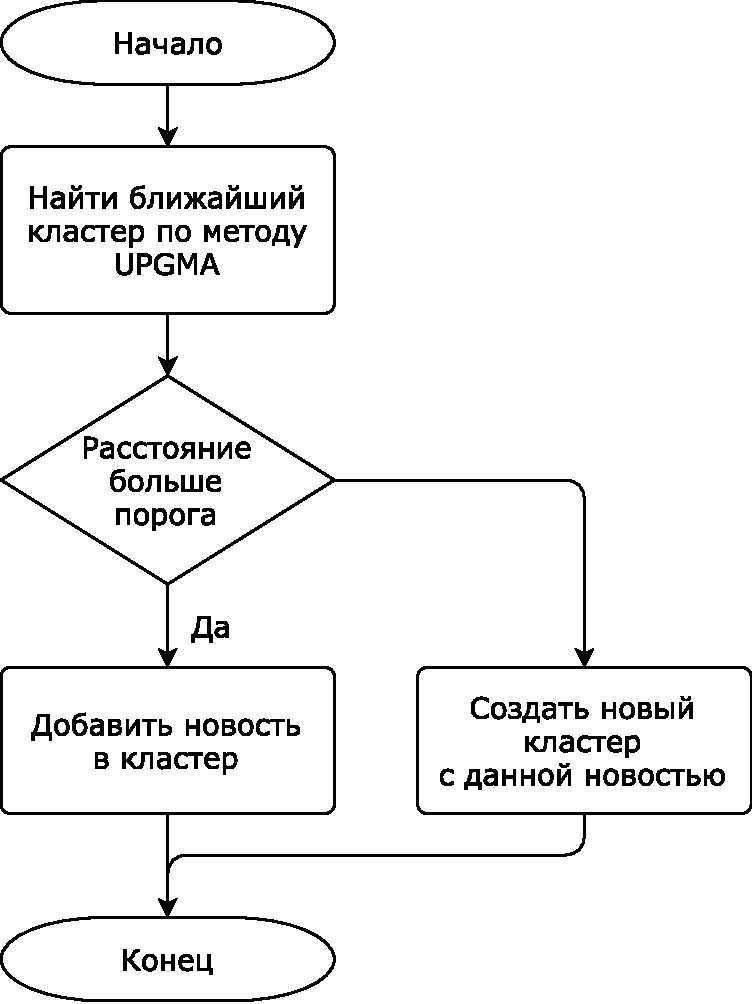
\includegraphics[width=.6\textwidth]{ica.pdf}
    \caption{Блок-схема ICA.}
    \label{fig:ica}
\end{figure}

На данном шаге проводится непосредственно кластеризация~--- объединение новостей в кластеры. Для этого используется алгоритм ICA (рис.~\ref{fig:ica}), выбранный в результате анализа, проведённого в разделе \ref{sssec:clustering-comparision}.

\subsection{Распространение оценки экспертов}
Последним шагом на данном этапе является распространение оценки экспертов. На входе шага имеем множество кластеров и множество экспертных оценок.

Для каждой экспертной оценки помечаем все новости в кластере как недостоверные с оценкой, пропорциональной расстоянию между экспертной новостью и рассматриваемой:
\begin{equation}
    s_y=s_x\cdot sim(x,y),
\end{equation}
где $s_x$ и $s_y$~--- вероятностные оценки недостоверности новостей $x$ и $y$, содержащихся в одном кластере.

\section{Ранжирование}
Заключительным этапом работы системы является ранжирование источников по степени доверия к новостям, публикуемым ими (рис.~\ref{fig:rater}).

\begin{figure}[h]
    \centering
    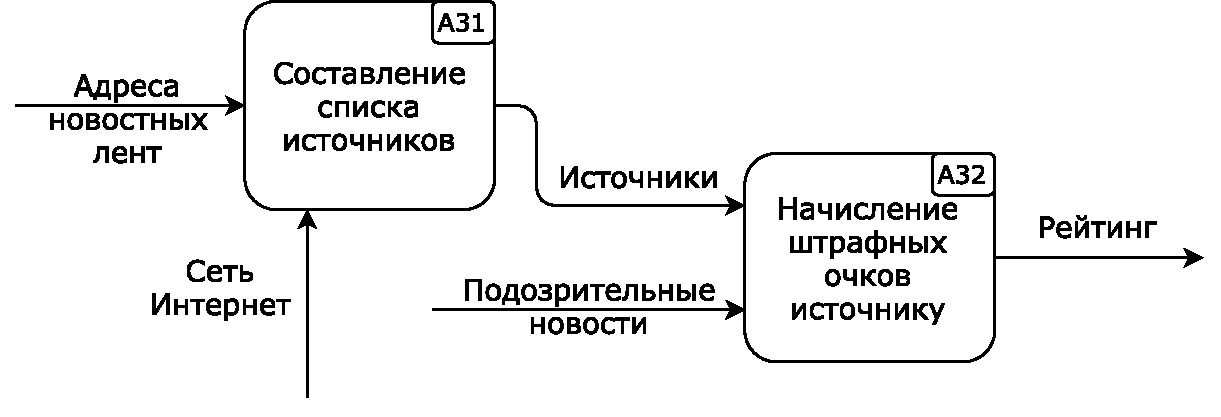
\includegraphics[width=.8\textwidth]{rater.pdf}
    \caption{Определение рейтинга.}
    \label{fig:rater}
\end{figure}

\subsection{Составление списка источников}
Список источников может быть получен из новостной ленты, поскольку каждая rss/atom-лента обязана содержать ссылку на сайт источника.

\subsection{Начисление штрафных очков источнику}
Данный шаг получает на вход список источников и список всех недостоверных статей с их оценками, полученными системой (либо от экспертов, либо в результате распространения экспертной оценки на этапе кластеризации).

Для формирования рейтинга используется подход, описанный в разделе \ref{ssec:simple-ranking}.
